%!TEX root = ../swiatlow_thesis.tex
\label{chapter:detector}

Though designed with eight potential interaction points, the LHC was eventually decided to serve collisions to four experiments: ATLAS, CMS, ALICE, and LHCb. ATLAS (A Toroidal LHC APparatus) and CMS (Compact Muon Solenoid) were designed as general purpose, high-precision, high-luminosity detectors, while ALICE was targeted towards analyzing heavy-ion collisions and LHCb would focus on $B$-physics. The data presented in this thesis was collected by the ATLAS experiment in $pp$ collisions at $\sqrt{s} = 8$~TeV in 2012. 

%2012 luminosity figure? Or in LHC section?

%%%%%%%%%%%%%%%%

\begin{figure}
\centering
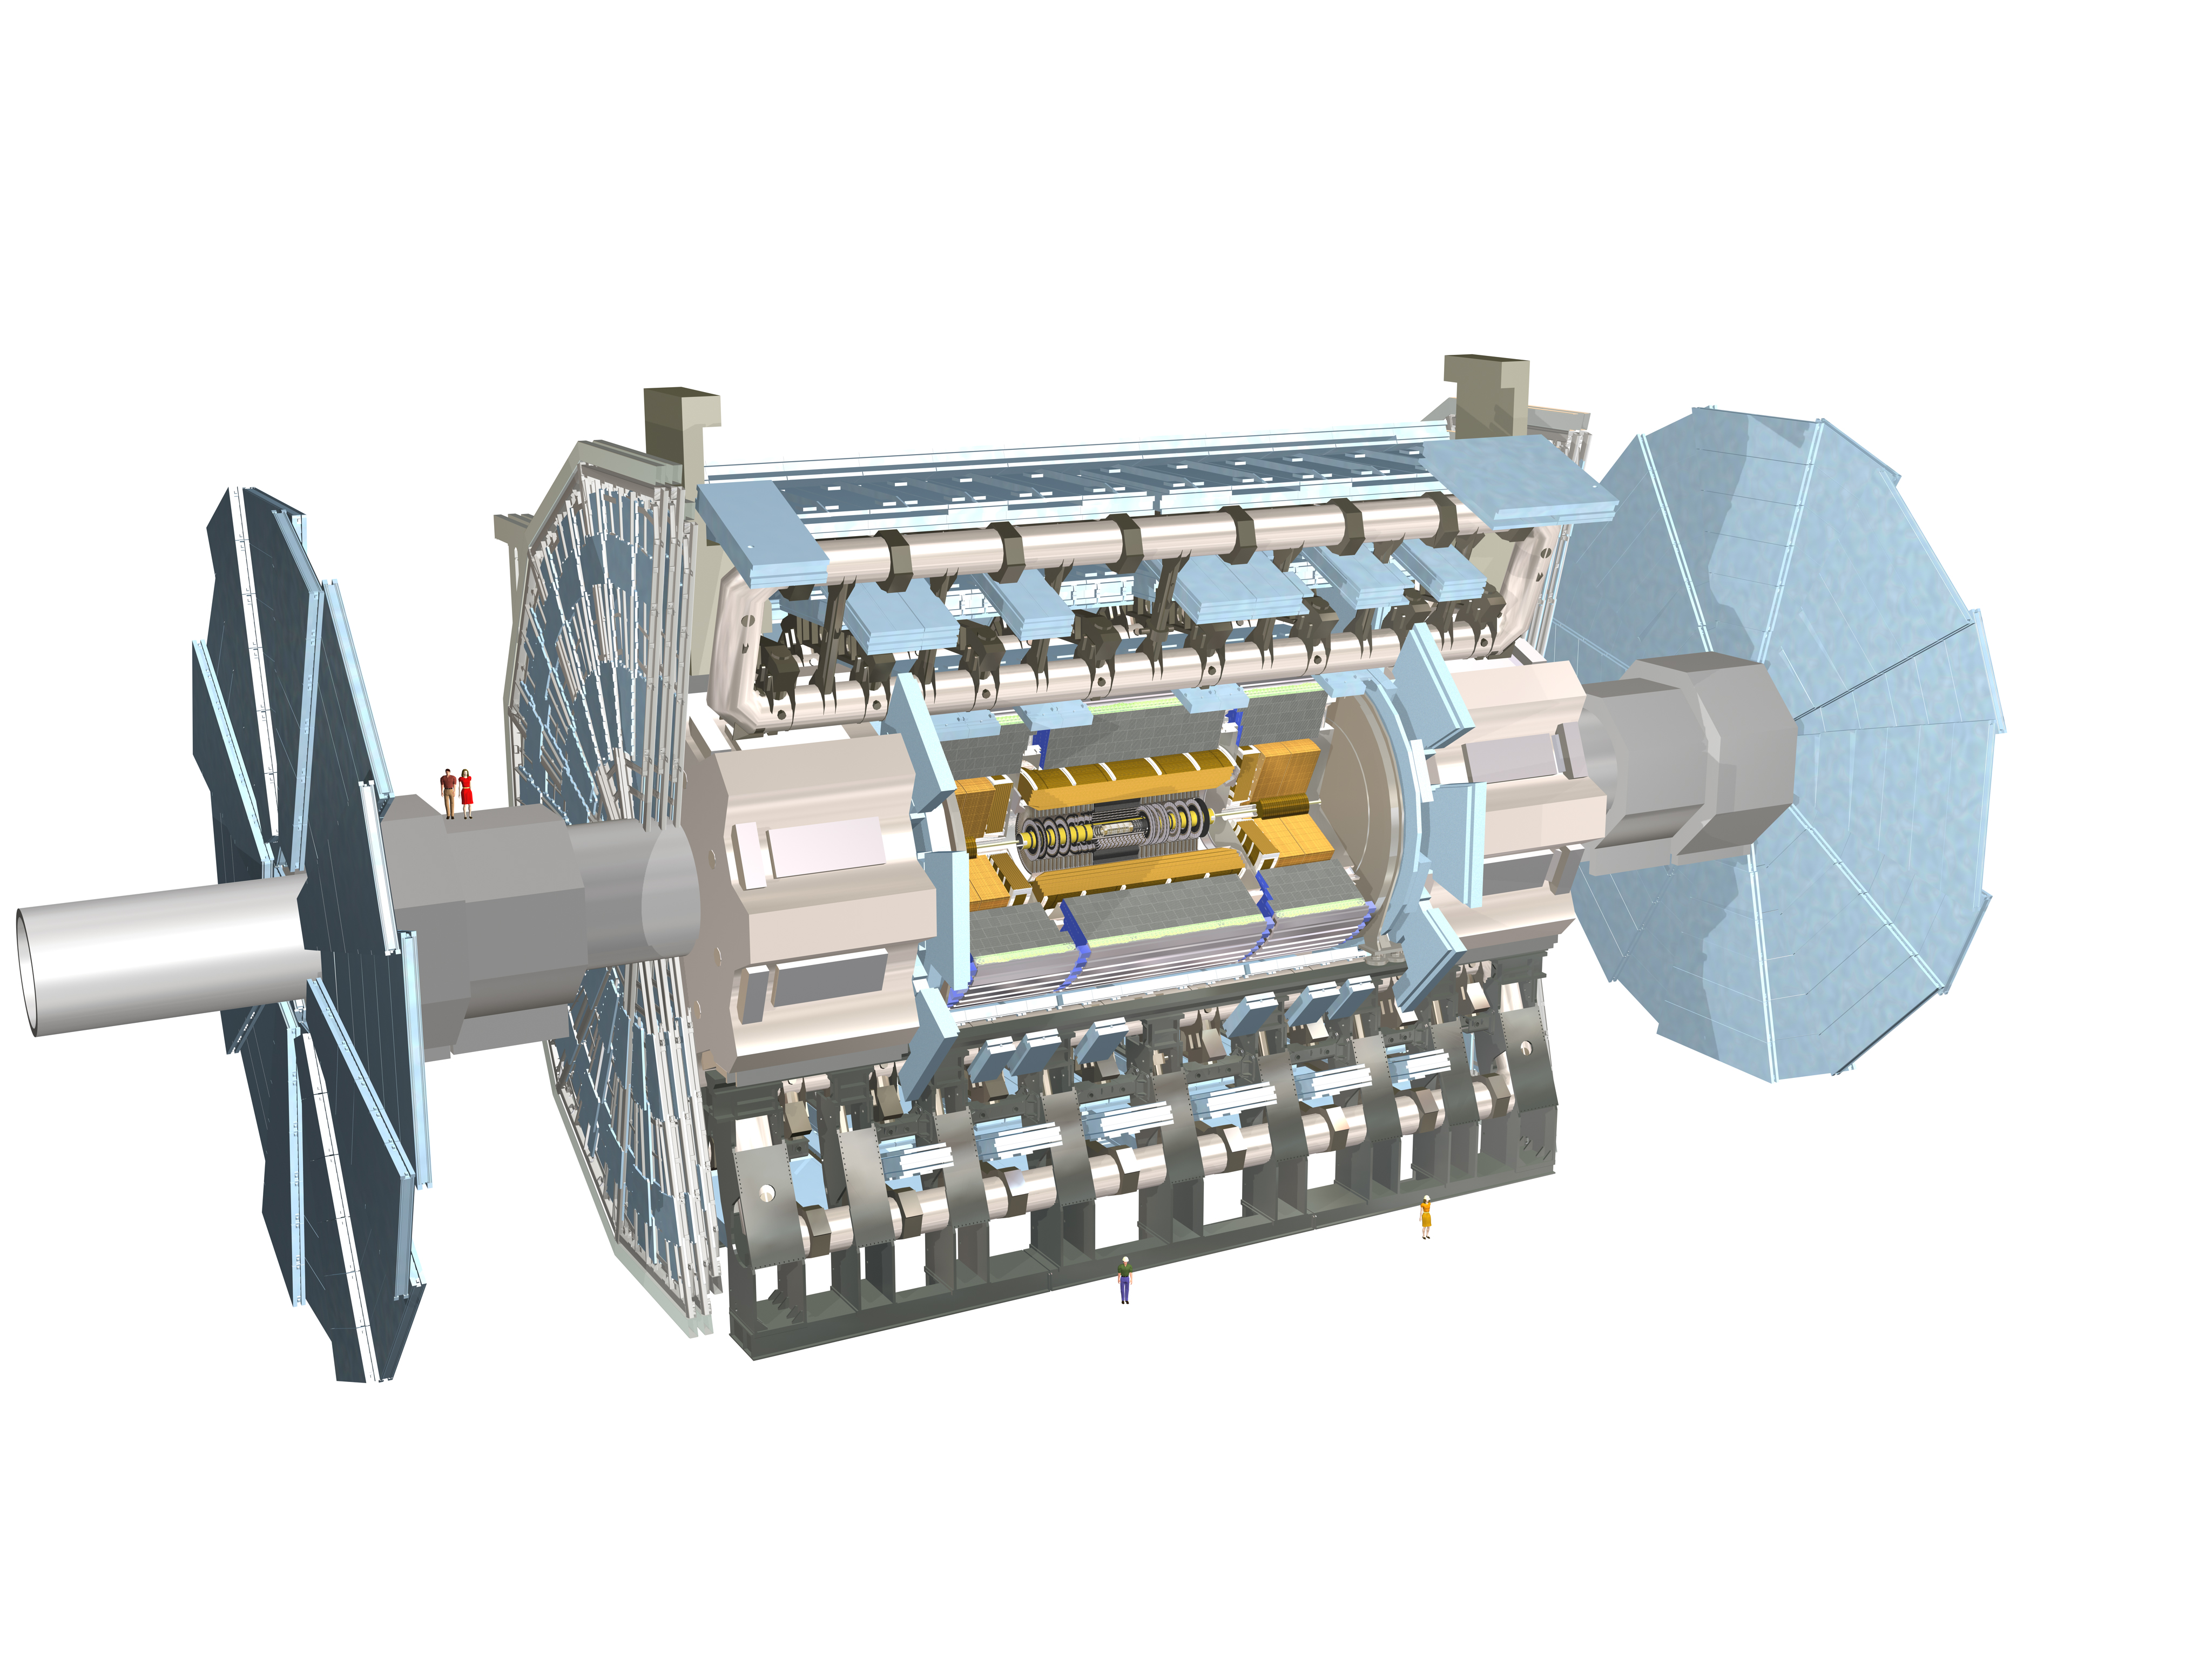
\includegraphics[width=0.7\textwidth]{atlas.jpg}
\label{fig:detector:atlas}
\caption{A computer-generated view of the ATLAS detector, with people for scale. Copyright CERN.}
\end{figure}

%%%%%%%%%%%%%%%% 


%Detector figure

\section{History}

The first public discussion of the proposals which became the ATLAS detector occurred in 1992 at the General Meeting on LHC Physics at Evian-les-Bains~\cite{Evian,EvianCourier}. At the time, four general purpose detectors (much like the four detector configuration in place at LEP) were seriously considered: EAGLE, ASCOT, CMS, and L3 (as an upgrade to the existing LEP detector, including a movable stage which would allow it to take data from both $e^+/e^-$ and $pp$ collisions). Several additional single purpose (heavy ion, neutrino, and $B$-physics) detectors were also proposed.

ATLAS emerged in a later 1992 Letter of Intent as a merger of the ASCOT and EAGLE collaborations~\cite{ATLAS-LoI}. ASCOT (Apparatus with SuperCOnducting Toroids) contributed the physically-defining feature of the secondary toroidal magnet system and standalone muon measurement system, as well as the tradition of using a tortured amalgamation of letters to form a name. EAGLE (Experiment for Accurate Gamma, Lepton and Energy measurements) on the other hand featured a stronger 2 T magnetic field, and inner-detector and calorimeter designs more similar to some of the final ATLAS systems. The detector described in the Letter of Intent already resembled ATLAS in many important ways, featuring the superconducting air-core toroids, accordion-shaped liquid Argon electromagnetic calorimeters, scintillating tile hadron calorimeters, and multi-design inner detector. \ref{fig:detector:earlyatlas} shows an early drawing of ATLAS from the Letter, and already the detector looks recognizable to its current form.

% Any citations on UA1 origins?

%%%%%%%%%%%%%%%%

\begin{figure}
\centering
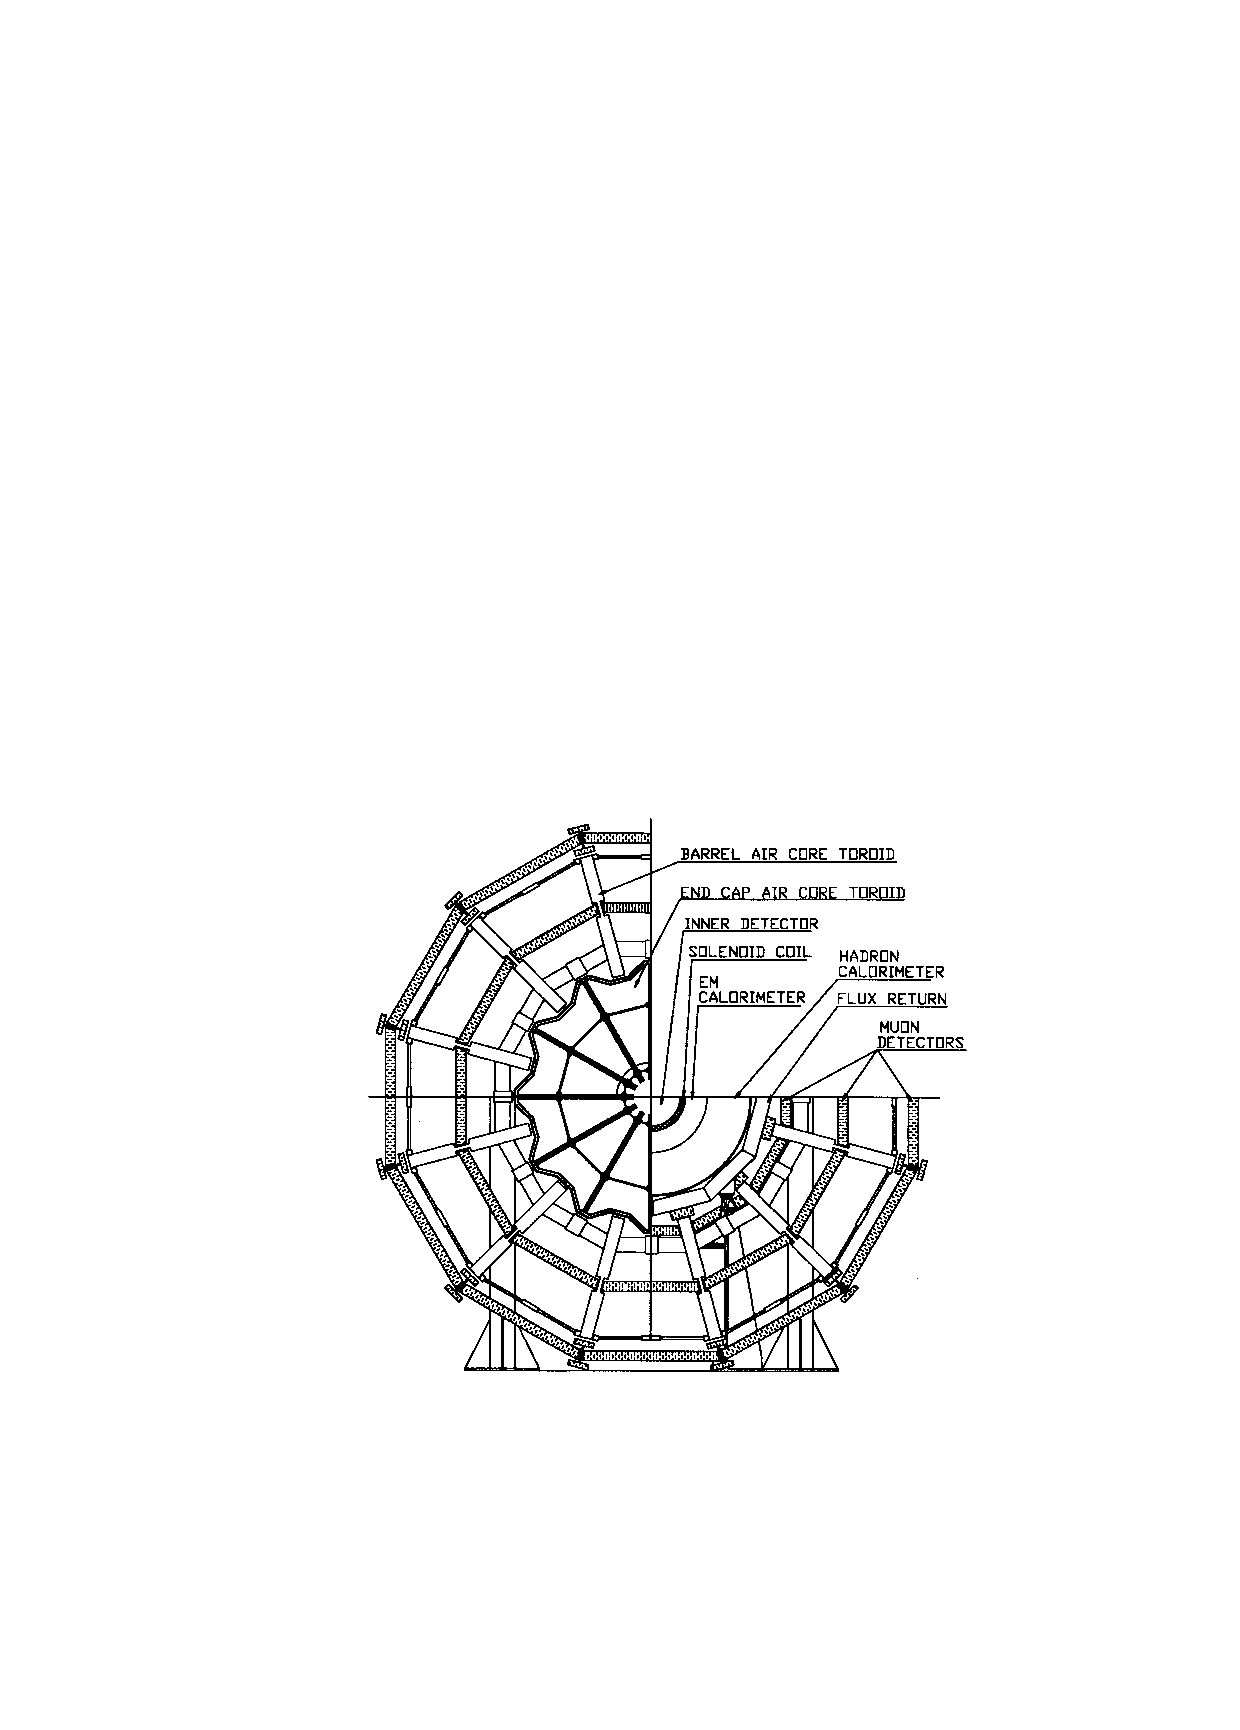
\includegraphics[width=0.7\textwidth]{early-atlas.pdf}
\label{fig:detector:earlyatlas}
\caption{An early view of a potential superconducting air-core toroid magnet system for the ATLAS detector from the 1992 Letter of Intent~\cite{ATLAS-LoI}.}
\end{figure}

%%%%%%%%%%%%%%%% 

\section{Inner Detector}

%%%%%%%%%%%%%%%%

\begin{figure}
\centering
\includegraphics[width=0.7\textwidth]{inner-detector.jpg}
\label{fig:detector:atlas}
\caption{A computer-generated view of the ATLAS inner detector, with relevant sizes of the detector marked out. Copyright CERN.}
\end{figure}

%%%%%%%%%%%%%%%% 

%%%%%%%%%%%%%%%%

\begin{figure}
\centering
\includegraphics[width=0.7\textwidth]{inner-detector-2.jpg}
\label{fig:detector:atlas}
\caption{A cut-out view of the ATLAS inner detector, showing the layers a particle would interact with as it passed outward from the collision point. Copyright CERN.}
\end{figure}

%%%%%%%%%%%%%%%% 

\subsection{Pixel Detector}

%%%%%%%%%%%%%%%%

\begin{figure}
\centering
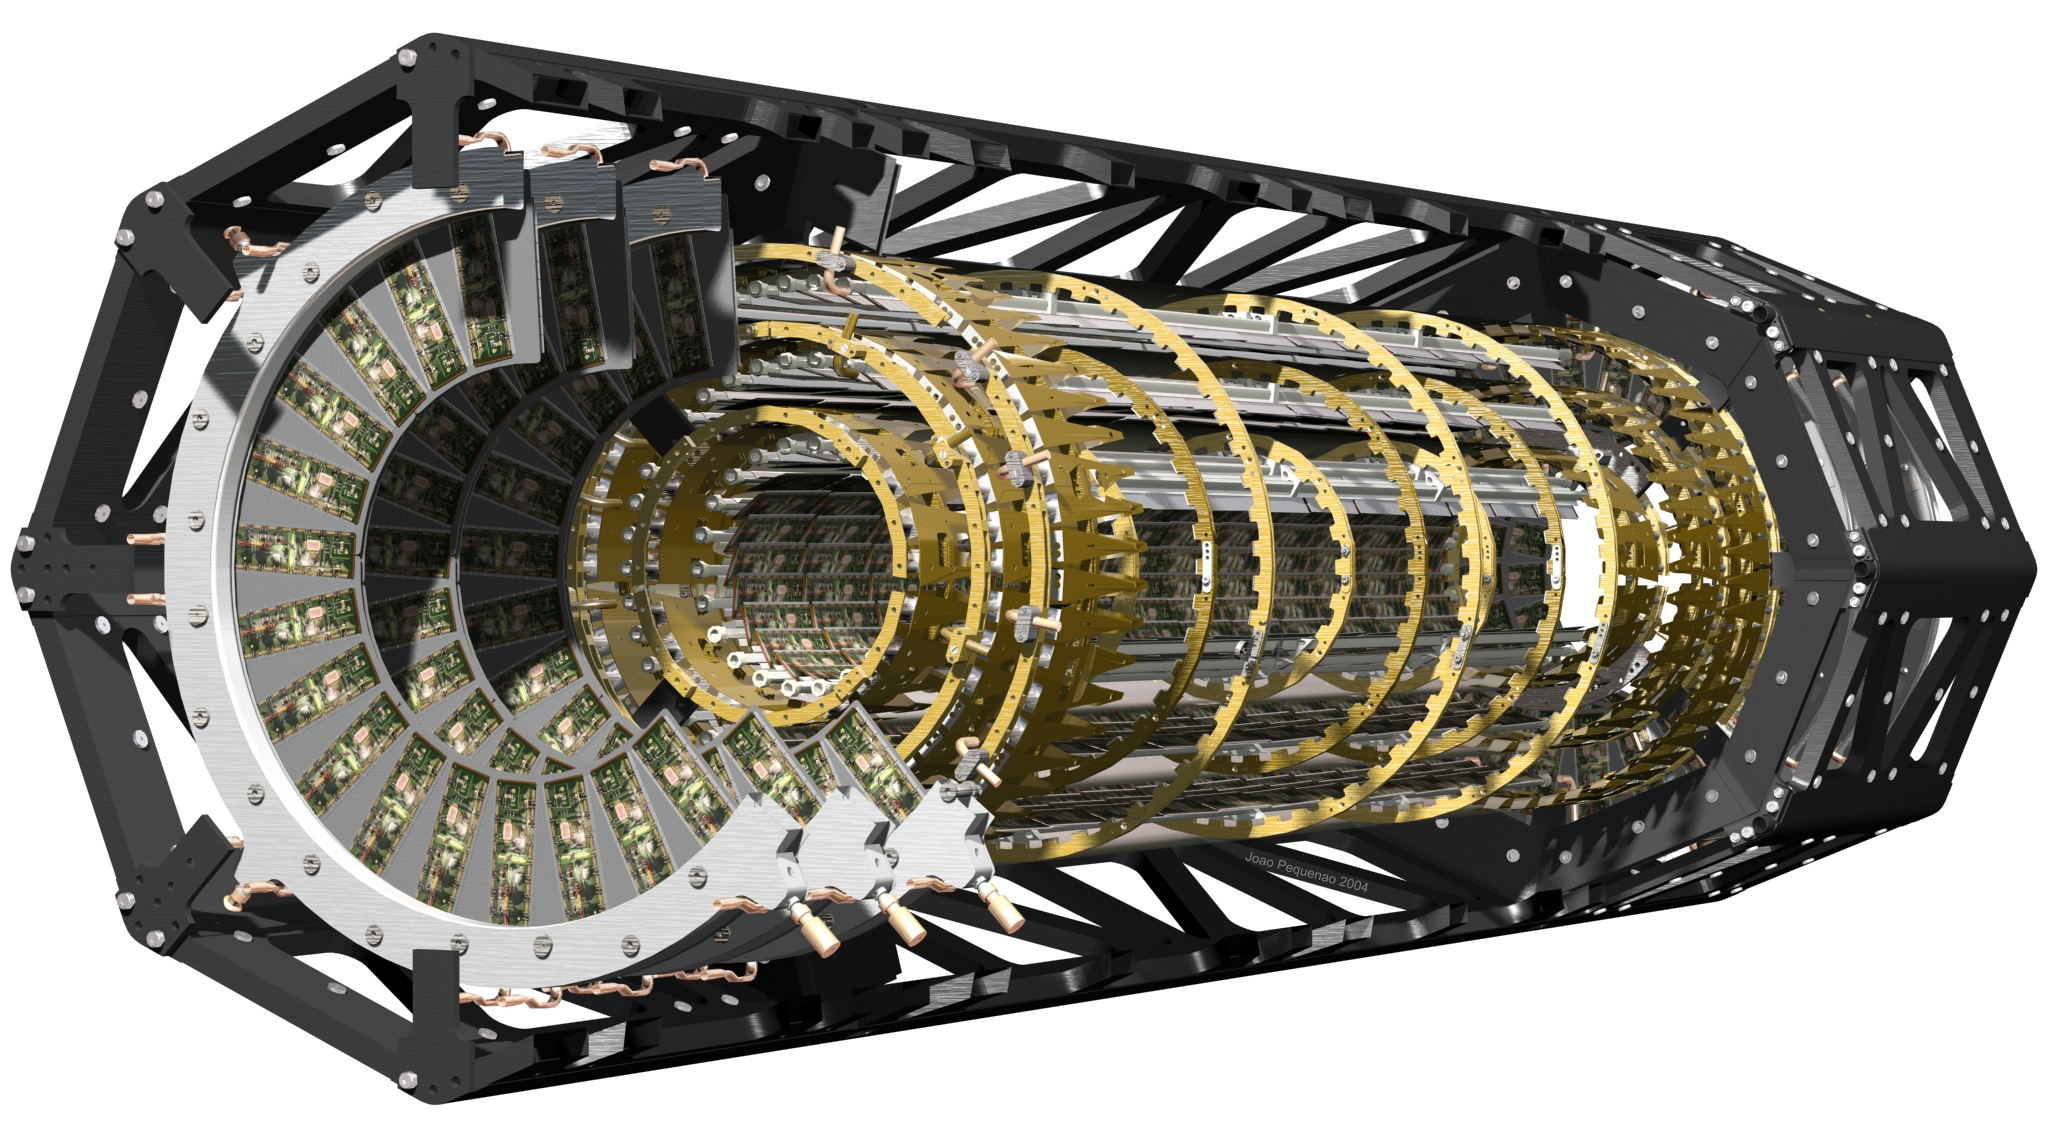
\includegraphics[width=0.7\textwidth]{pixel.jpg}
\label{fig:detector:atlas}
\caption{A computer-generated view of the ATLAS pixel detector. Copyright CERN.}
\end{figure}

%%%%%%%%%%%%%%%% 



\subsection{Silicon Strip Tracker}


%%%%%%%%%%%%%%%%

\begin{figure}
\centering
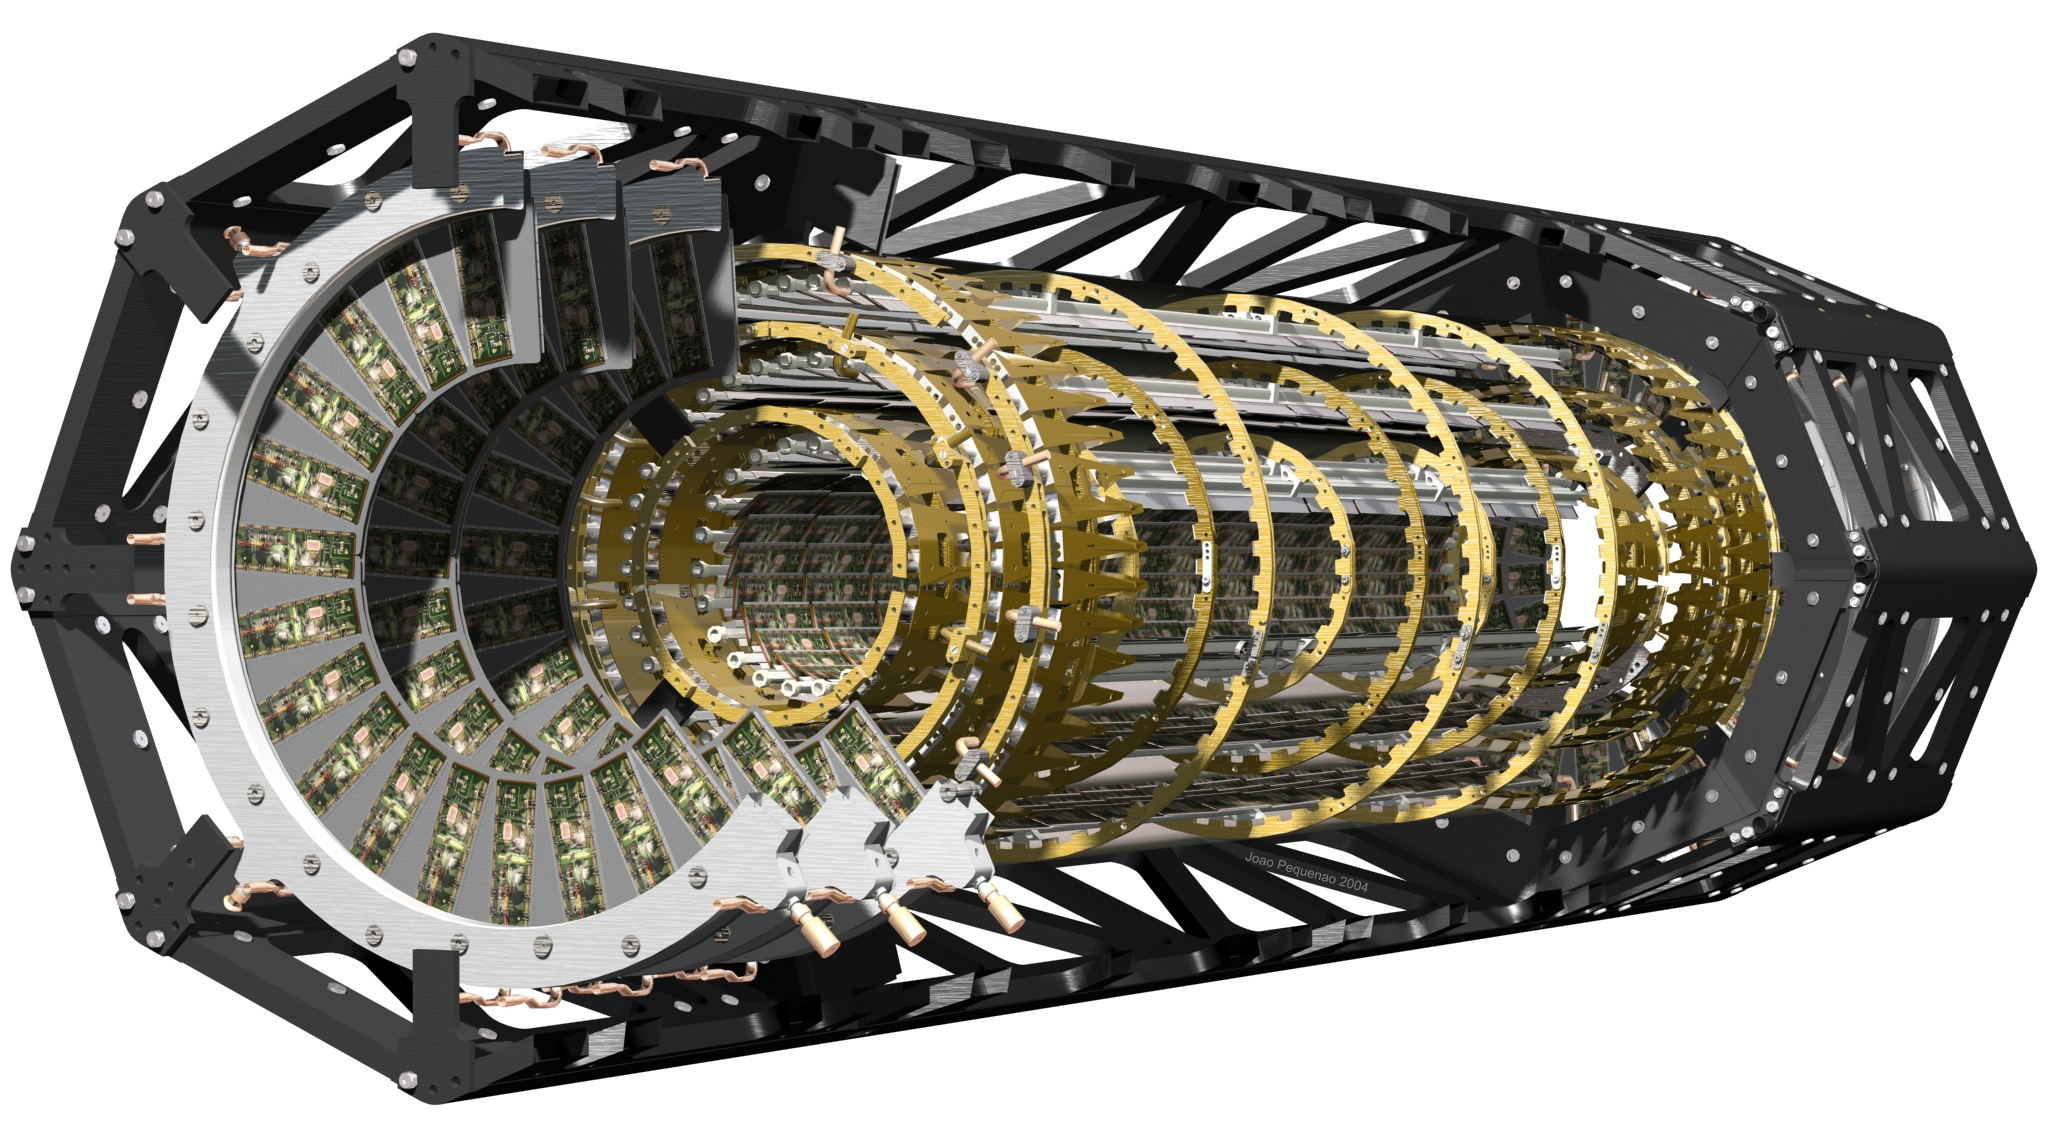
\includegraphics[width=0.7\textwidth]{pixel.jpg}
\label{fig:detector:atlas}
\caption{A photograph of one segment of the ATLAS SCT barrel system. Copyright CERN.}
\end{figure}

%%%%%%%%%%%%%%%% 

\subsection{Transition Radiation Tracker}

%%%%%%%%%%%%%%%%

\begin{figure}
\centering
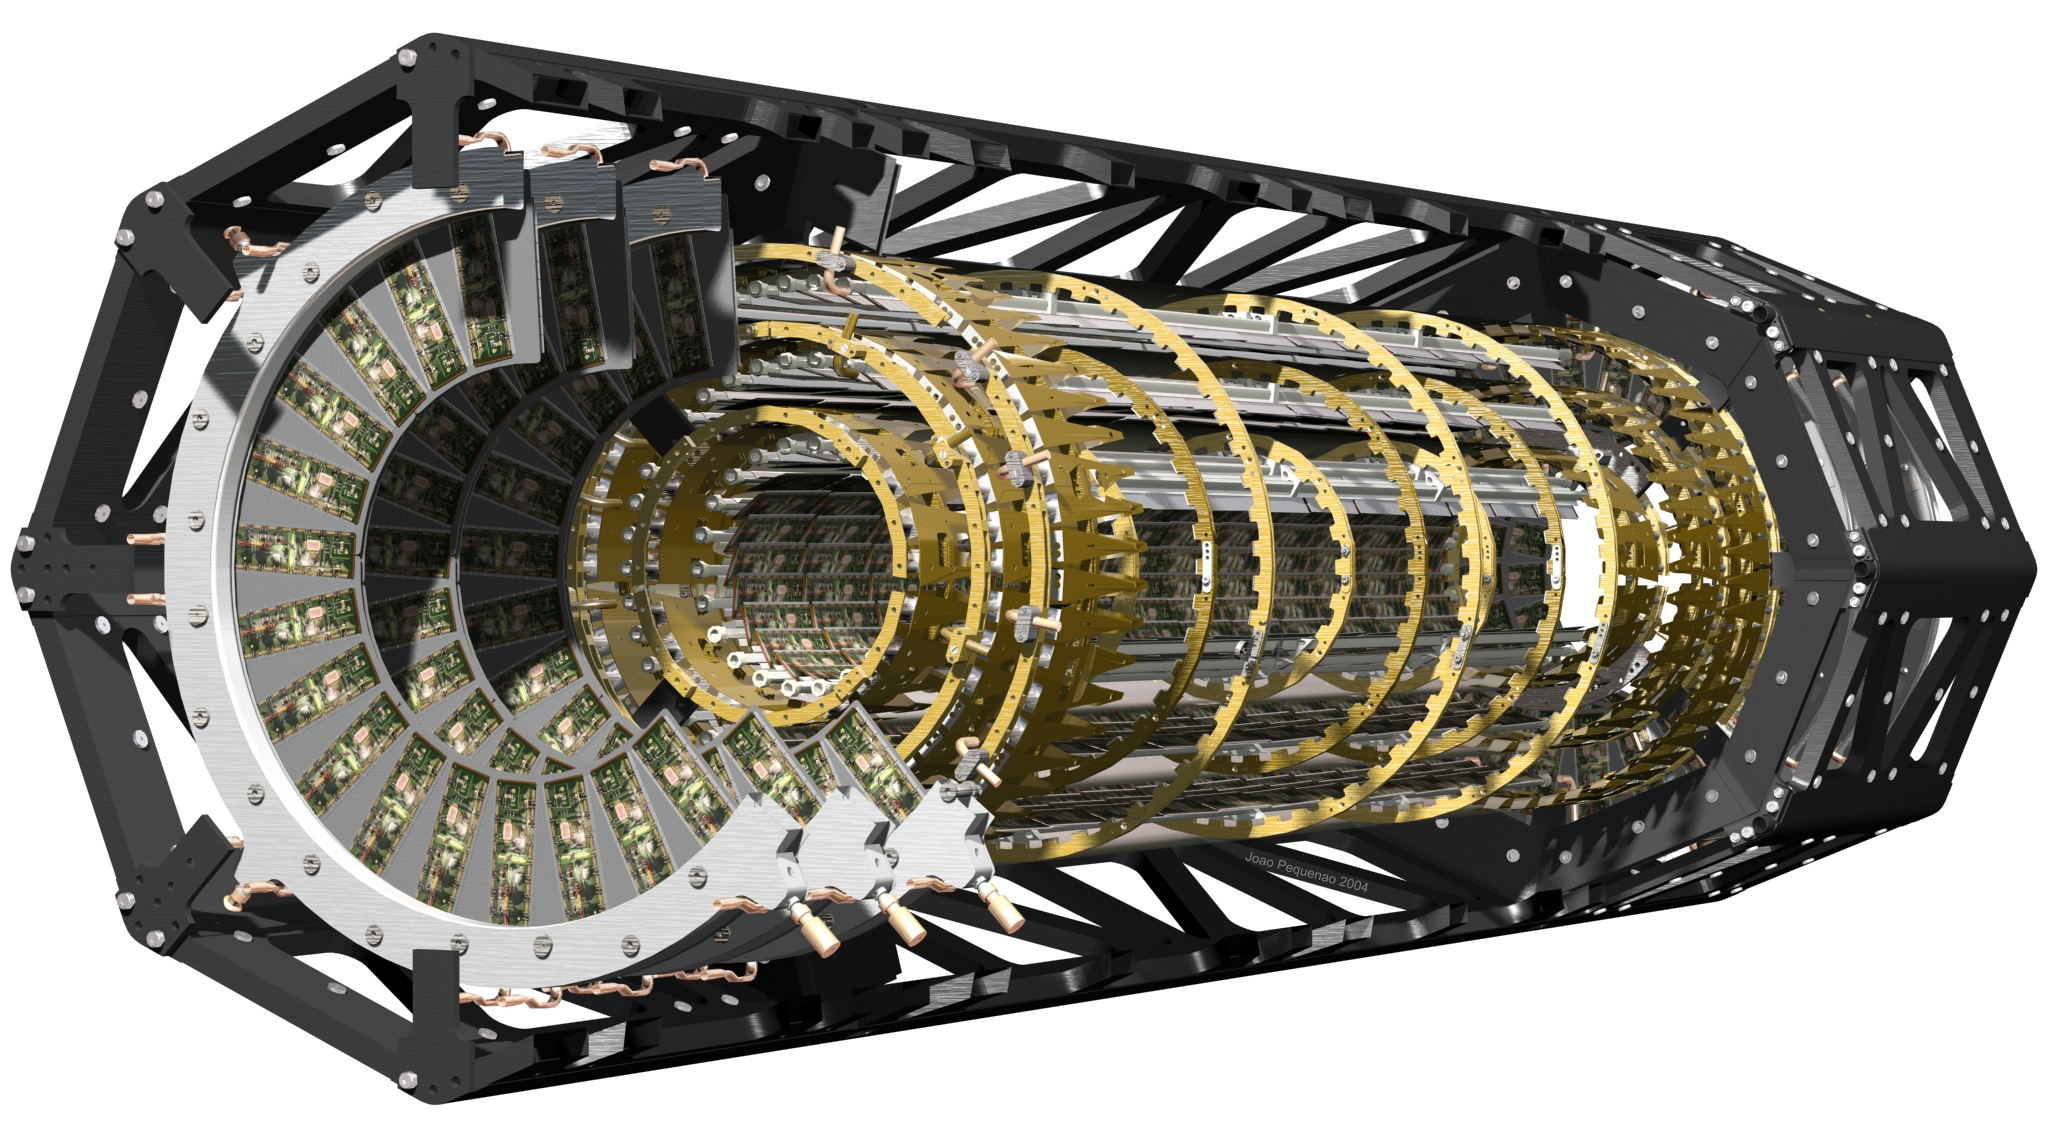
\includegraphics[width=0.7\textwidth]{pixel.jpg}
\label{fig:detector:atlas}
\caption{A photograph of the ATLAS TRT system during testing. Copyright CERN.}
\end{figure}

%%%%%%%%%%%%%%%% 

\section{Calorimeters}

\subsection{Electromagnetic Calorimeter}

\subsection{Hadron Calorimeter}

\section{Muon Spectrometer}

\section{Triggering}

\section{Data Quality}